\chapter{Romberg quadrature}

\section{The algorithm}

Let \(f:[a,b] \rightarrow \R\) be a function and \(I\coloneqq \int_a^bf(x)dx\). The {\it trapezoidal rule} is a method for approaching \(I\) which works as follows: Let \(a = t_0 < t_1 < \cdots < t_n = b\) be a subdivision of \([a,b]\). On each of the intervals \([t_{i-1},t_i]\) we approximate \(\int_{t_{i-1}}^{t_i}f(x)dx\) by the area of a trapezoid with verticies \((t_{i-1},0),\,(t_{i-1}, f(t_{i-1})),\,(t_i,f(t_i)),\, (t_i,0)\) i.e. by \(\frac{1}{2}(t_i - t_{i-1})(f(t_{i-1}) + f(t_i))\). Hence we approximate \(I\) by 

\[
I = \sum_{i=1}^n \int_{t_{i-1}}^{t_i}f(x)dx \approx \sum_{i=1}^n\frac{1}{2}(t_i - t_{i-1})(f(t_{i-1}) + f(t_i)).
\]
If \(t_i - t_{i-1} = \frac{1}{n}(b-a)\eqqcolon h\) for each \(i\) then the above estimate becomes
\begin{equation}\label{trapezoidal}
I \approx h \left(\frac{1}{2}(f(a) + f(b)) + \sum_{i=1}^{n-1}f(a + ih)\right)
\end{equation}
We define \(T_f(h)\) as the right hand side in (\ref{trapezoidal}) for all \(h\in \{(b-a)/n\mid n \in \Z_+\ldots\}\eqqcolon \Hset\).\\

Let \(F:[0, n]\rightarrow \R\) be a \(2k+1\) times continuously differentiable function, \(n\) a positive integer. Then by Euler's summation formula (see formula 298 in \cite{kn}) we have
\begin{equation}
\sum_{i=0}^nF(i) = \int_0^nF(x)dx + \frac{1}{2}(F(0) + F(n)) + \sum_{i=1}^k\frac{B_{2i}}{(2i)!}(F^{(2i-1)}(n) - F^{(2i-1)}(0)) + R_k
\end{equation}
where \(R_k = \int_0^nP_{2k+1}(x)F^{(2k+1)}(x)dx\), \(B_m\) are the {\it Bernoulli numbers} and \(P_m\) the {\it Bernoulli polynomials.} If we let \(F(x)\coloneqq f(a + xh)\) then we get the following asymptotic expansion for the trapezoidal rule:

\begin{theorem}
Let \(f:[a,b] \rightarrow \R\) be \(2k+1\) times continuously differentiable and \(h \coloneqq (b-a)/n\). Then 
\begin{equation}
T_f(h) = I + \sum_{i=1}^k\frac{B_{2i}}{(2i)!}(f^{(2i-1)}(b) - f^{(2i-1)}(a))h^{2i} + h^{2k+1}R_k(h)
\end{equation}
where
\begin{equation}
R_k(h) = \int_a^bP_{k+1}\left(n\frac{x-a}{b-a}\right)f^{(2k+1)}(x)dx. 
\end{equation}
\end{theorem}

The following code is a trivial implementation of the trapezoidal rule. The {\it TrapezoidalRule} class in an implementation of the abstract class {\it Scheme} which represents a numerical scheme or method, which has asymptotic expansion in \(h^p\). The Scheme class has a method named {\it apply} which takes in a problem to which the scheme is applied to. The argument \(m\) in the apply-method is the number of subintervals that should be used.

\begin{minted}[tabsize=2, fontsize=\footnotesize]{python}
class TrapezoidalRule(Scheme):
    def __init__(self):
        super(TrapezoidalRule, self).__init__(2)

    def apply(self, inte, m):
        (a,b) = inte.interval
        h = (b - a) / m
        I = 0.5 * (inte.f(a) + inte.f(b))
        for i in range(1, m):
            I += inte.f(a + i * h)

        return I * h
\end{minted}

Assume that we have computed the value of \(T_f(h)\) for \(h = h_1,\ldots,h_k\) and we want to extrapolate to zero, i.e. we want to compute the value at zero of the interpolation polynomial in \(h^2\) for \((h_i^2,T_f(h_i)\), \(i=1,\ldots,k\). Denote by \(T_{ij}\) the value at zero of the polynomial of degree \(j-1\) in \(h^2\) which goes through \((h_{i-j+1}^2, T(h_{i-j+1})),\ldots,(h_i^2,T(h_i))\). The Neville scheme gives us the following algorithm for computing \(T_{ij}\), \(1\leq j\leq i\leq k\), recursively:

\begin{enumerate}
    \item \(T_{i1} \coloneqq T_f(h_i)\) for \(i = 1,\ldots,k\).
    \item \(T_{ij} \coloneqq T_{i,j-1} + \frac{T_{i,j-1} - T_{i-1,j-1}}{\left(\frac{h_{i-j+1}}{h_i}\right)^2 - 1}\) for \(2\leq j\leq i\).
\end{enumerate}

\section{Numerical experiments}

In this section we are going to apply Romberg quadrature to various functions and also try different sequences. We will analyse how different sequences perform in the sense that we want to measure how many function evaluations we need to attain a prescribed precision.\\

We will try various functions and the following sequences:
\begin{itemize}
    \item The harmonic sequence: \(a_n = n\), \(n > 0\).
    \item The Romberg sequence: \(a_n = 2^{n-1}\), \(n\geq 1\).
    \item The Bulirsch sequence: \(a_1 = 1\), \(a_2 = 2\), \(a_3 = 3\) and \(a_{n+2} = 2\cdot a_n\) for \(n\geq 2\). Its first elements are 
    \[
    1,\, 2,\, 3,\, 4,\, 6,\, 8,\, 12,\, 16,\, 24,\, 32,\ldots
    \]
\end{itemize}

Suppose that we are approximating the integral \(I\coloneqq \int_a^b f(x)dx\) using Romberg quadrature. We will use the stepsizes \(h_k\coloneqq (b-a)/a_k\) for the extrapolation. Let \(T_{ij}\), \(i\geq 0\) and \(j\leq i\) be the extrapolation table we get and \(\varepsilon_k \coloneqq |T_{kk}-I|\) be the error on the diagnoals. Let \(N_k\) be the number of function evaluations needed to compute \(T_{kk}\). We will use \(N_k\) as the measurement of computational effort as mentioned in section 1.3 and we will try to fit the exponential convergence model introduced there. We will also plot the logarithm of the error against the number of extrapolation steps. Note that \(N_k = \sum_{i=1}^k(a_i + 1)\) where \((a_i)\) is our sequence, so in case of the Harmonic sequence, we have \(N_n = n(n+3)/2 \approx n^2/2\) for \(n\) large. Hence if \(\varepsilon_n \sim A\exp(-cN_n^q)\) then 
\[
\varepsilon_n \sim A\exp(-c/2^qn^{2q})
\]
for \(n\) large. Thus if the error converges exponentially with the number of function evaluations, it will also converge exponentially with the number of extrapolation steps, and the exponent in the latter fitting will be twice the parameter from the former.\\

If our sequence is the Romberg sequence then \(N_k = \sum_{i=1}^k (2^{i-1} + 1) = 2^k + k - 1 \approx 2^k\) for \(k\) large, so if \(\varepsilon_k\sim A \exp(-cN_k^q)\) then 
\[
\varepsilon_k \sim A\exp(-c 2^{kq}) 
\]
for \(k\) large, which is not exponential convergence. Hence possibilities of having exponential convergence in the number of steps and in the number of evaluations are mutually exclusive for the Romberg sequence.\\

For the model fitting we will plot the logarithm of the error against the number of function evaluations  and the number of extrapolation steps. Then we will try to fit the points on curve of a function of the form \(t\mapsto b - ct^q\) and we will report the mean and relative variance of \(A\coloneqq e^b\), \(c\) and \(q\). We will also provide the plot of the base \(10\) logarithm of the error against the number of function evaluations. \\

We conduct the experiments in Python 3 and use the high precision arithmetic library mpmath for all the computations. The precision will be set to \(500\) significant digits so will not have to worry about numerical instabilities.\\

Now we will consider the results of the experiments.

\subsection{Cosine squared}
The first function we are going to try is
\[
f: [0, 1]\rightarrow \R, \quad f(x) \coloneqq \cos^2(x)
\]
which is entire.

%cos^2(x)
\begin{figure}[H]
\centering
\begin{minipage}{0.45\textwidth}
\centering
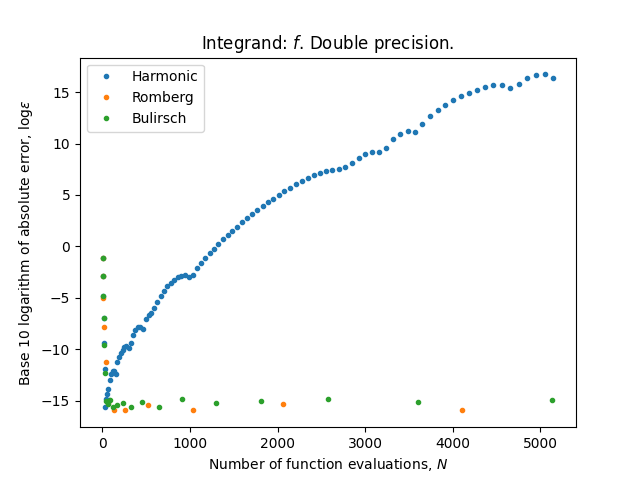
\includegraphics[scale=0.45]{../results/romberg_plots/cos_squared.png}
\end{minipage}
\begin{minipage}{0.45\textwidth}
\centering
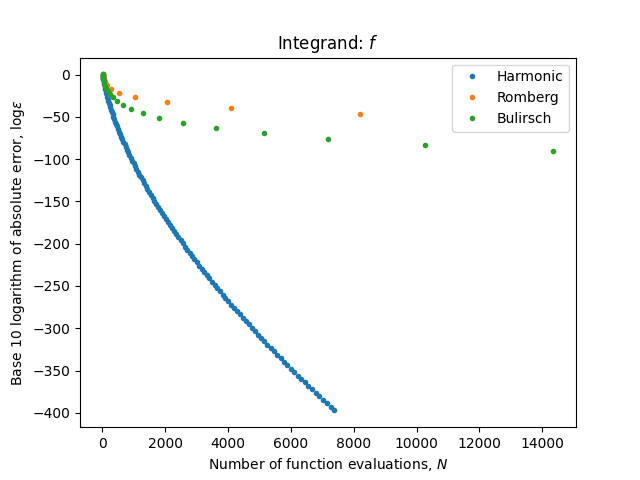
\includegraphics[scale=0.45]{../results/romberg_plots/cos_squared_hp.png}
\end{minipage}
\end{figure}

\begin{figure}[H]
\centering
\begin{minipage}{0.45\textwidth}
\centering
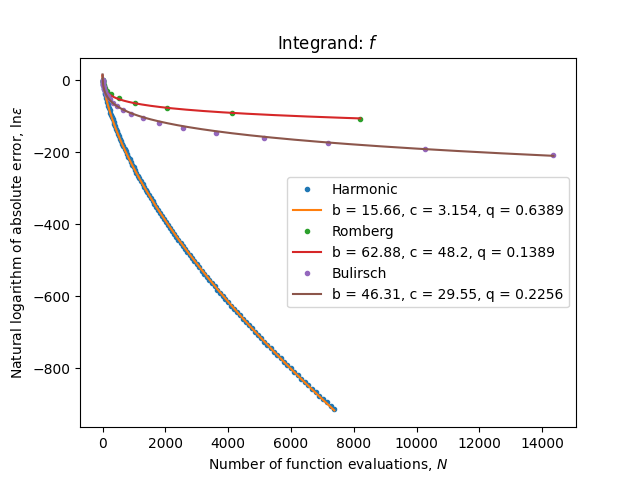
\includegraphics[scale=0.45]{../results/romberg_plots/cos_squared_hp_trend.png}
\end{minipage}
\begin{minipage}{0.45\textwidth}
\centering
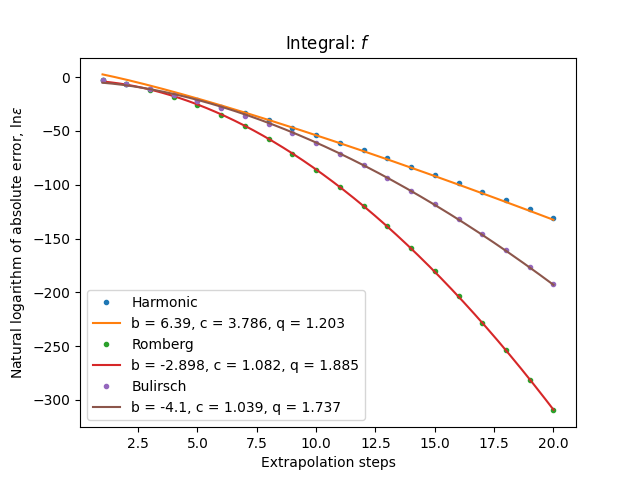
\includegraphics[scale=0.45]{../results/romberg_plots/cos_squared_hp_steps.png}
\end{minipage}
\end{figure}

\begin{figure}[H]
\centering
\begin{minipage}{0.45\textwidth}
\centering
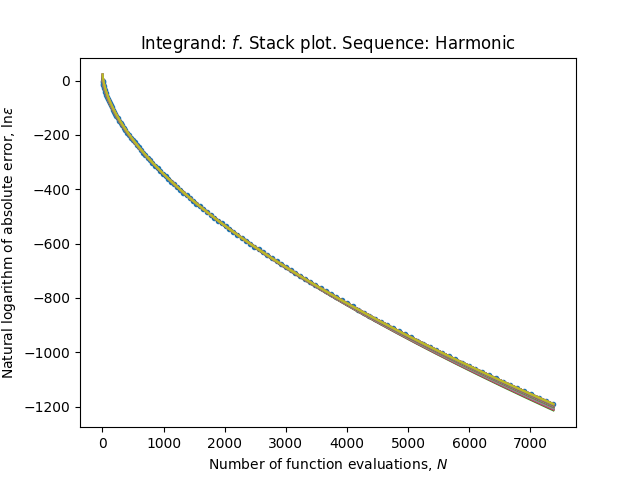
\includegraphics[scale=0.45]{../results/romberg_plots/cos_squared_hp_harmonic_stack.png}
\end{minipage}
\begin{minipage}{0.45\textwidth}
\centering
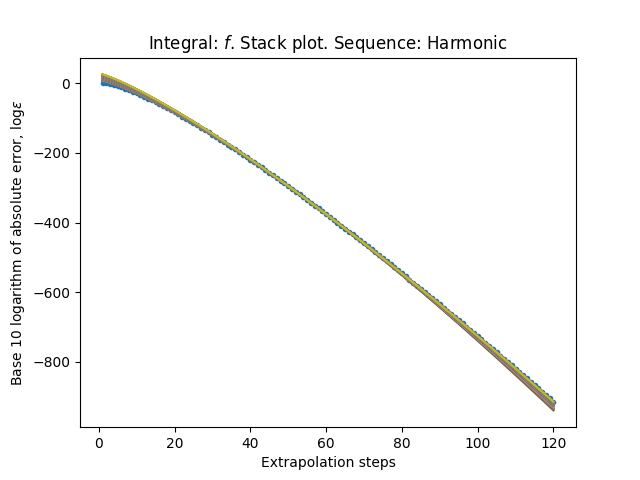
\includegraphics[scale=0.45]{../results/romberg_plots/cos_squared_hp_harmonic_steps_stack.png}
\end{minipage}
\end{figure}

\begin{figure}[H]
\centering
\begin{minipage}{0.45\textwidth}
\centering
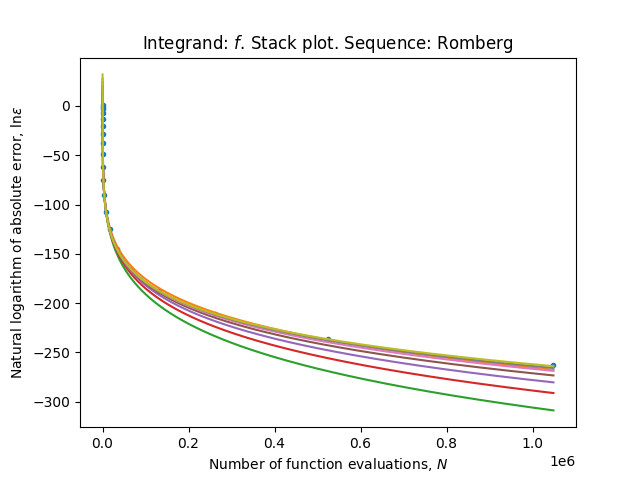
\includegraphics[scale=0.45]{../results/romberg_plots/cos_squared_hp_romberg_stack.png}
\end{minipage}
\begin{minipage}{0.45\textwidth}
\centering
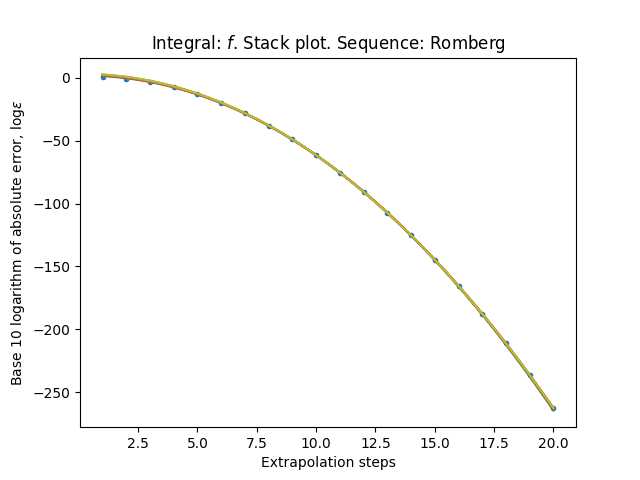
\includegraphics[scale=0.45]{../results/romberg_plots/cos_squared_hp_romberg_steps_stack.png}
\end{minipage}
\end{figure}

\begin{figure}[H]
\centering
\begin{minipage}{0.45\textwidth}
\centering
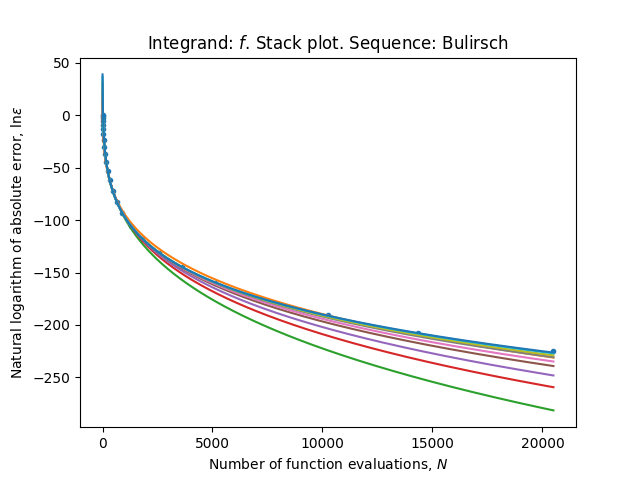
\includegraphics[scale=0.45]{../results/romberg_plots/cos_squared_hp_bulirsch_stack.png}
\end{minipage}
\begin{minipage}{0.45\textwidth}
\centering
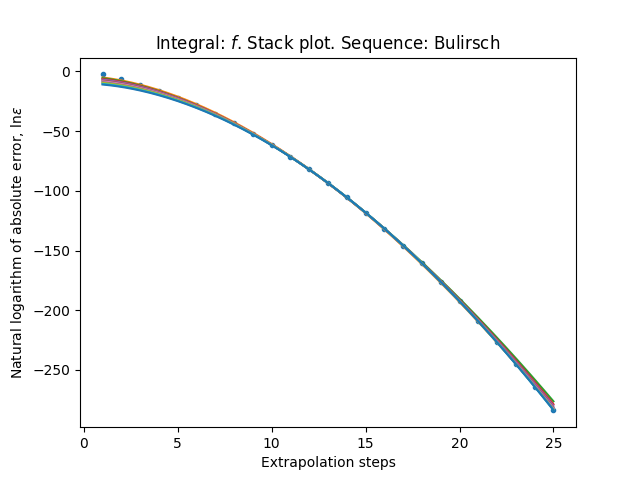
\includegraphics[scale=0.45]{../results/romberg_plots/cos_squared_hp_bulirsch_steps_stack.png}
\end{minipage}
\end{figure}

\begin{table}[H]
    \centering
    \small
    \begin{tabular}{c||c|c|c|c|c|c|c|c}
Sequence & \(A\)-mean & \(A\)-var & \(c\)-mean & \(c\)-var & \(q\)-mean & \(q\)-var & \(\rho_{\operatorname{lin}}\) & \(\rho_{\ln}\)\\\hline
\rowcolor{yellow}
Harmonic & \(8.644\cdot 10^{12}\) & \(7.493\) & \(5.843\) & \(0.004665\) & \(0.5999\) & \(0.00017\) & \(1.605\cdot 10^7\) & \(6.464\cdot 10^{-6}\) \\
\rowcolor{red}
Romberg & \(1.071\cdot 10^{73}\) & \(6\) & \(95.86\) & \(0.06674\) & \(0.1125\) & \(0.01945\) & \(1.14\cdot 10^7\) & \(0.0003937\) \\
\rowcolor{red}
Bulirsch & \(3.78\cdot 10^{76}\) & \(7.998\) & \(87.35\) & \(0.1063\) & \(0.164\) & \(0.03428\) & \(2.502\cdot 10^{10}\) & \(0.0007942\) \\
\rowcolor{yellow}
Harmonic & \(8.372\cdot 10^7\) & \(6.367\) & \(4.002\) & \(0.003408\) & \(1.193\) & \(0.0001069\) & \(2.727\cdot 10^4\) & \(3.325\cdot 10^{-6}\) \\
\rowcolor{green}
Romberg & \(0.0127\) & \(0.6464\) & \(1.015\) & \(0.002443\) & \(1.904\) & \(7.669\cdot 10^{-5}\) & \(0.5932\) & \(1.117\cdot 10^{-5}\) \\
\rowcolor{green}
Bulirsch & \(0.002302\) & \(2.227\) & \(0.9216\) & \(0.01377\) & \(1.771\) & \(0.0004207\) & \(0.8609\) & \(3.924\cdot 10^{-5}\) \\
    \end{tabular}
    \label{tab:my_label}
\end{table}

We see that the harmonic sequence performes best, then Bulirsch and then Romberg. In standard double precision arithmetic, we get down to machine level precision using Romberg or Bulirsch, but we are like \(2\) digits from there, using the harmonic sequence.\\

For the Romberg and Bulirsch sequence we clearly have exponential convergence in the number of steps but not in the number of evaluations.\\

For the harmonic sequence we get unreasonbly large values of \(A\) and we can see from the stack plots that the fitting is not so stable.\\

\subsection{Function with poles}

Now we will consider the following function:
\[
g_a: [-1, 1] \rightarrow \R, \quad g_a(x) \coloneqq \frac{1}{a^2 + x^2},\, a > 0
\]

\subsubsection{\(a = 1\)}

\begin{figure}[H]
\centering
\begin{minipage}{0.45\textwidth}
\centering
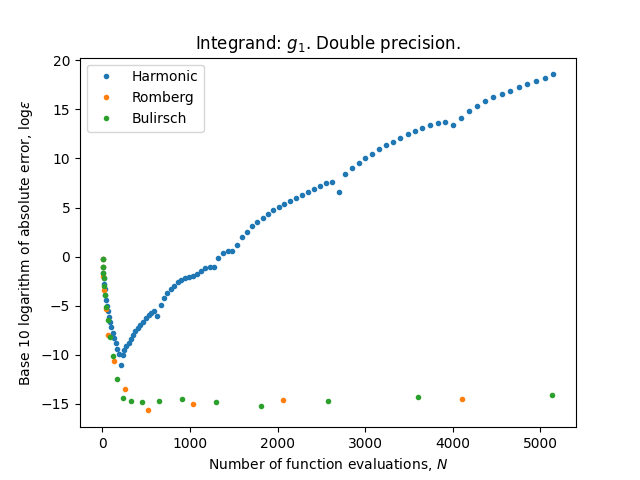
\includegraphics[scale=0.45]{../results/romberg_plots/g_one.png}
\end{minipage}
\begin{minipage}{0.45\textwidth}
\centering
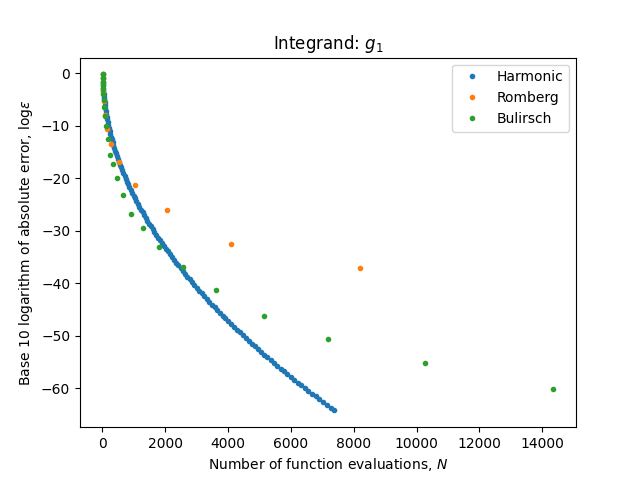
\includegraphics[scale=0.45]{../results/romberg_plots/g_one_hp.png}
\end{minipage}
\end{figure}

\begin{figure}[H]
\centering
\begin{minipage}{0.45\textwidth}
\centering
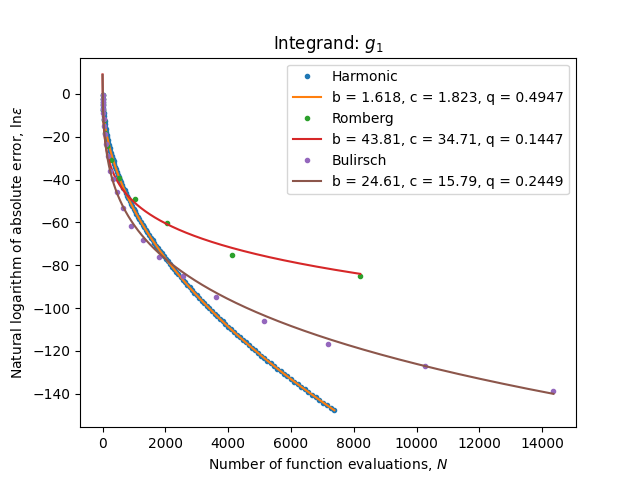
\includegraphics[scale=0.45]{../results/romberg_plots/g_one_hp_trend.png}
\end{minipage}
\begin{minipage}{0.45\textwidth}
\centering
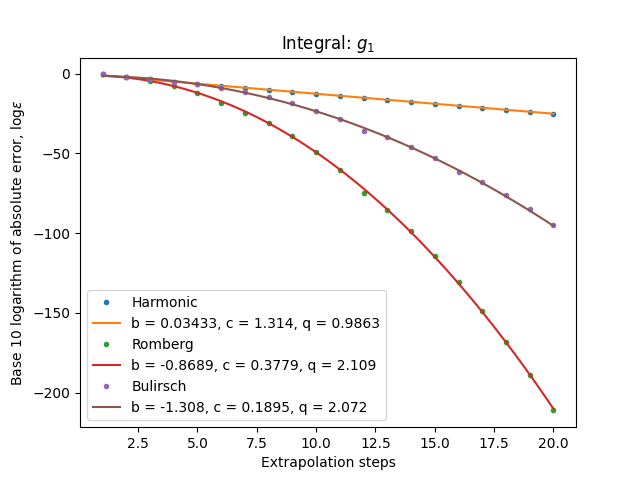
\includegraphics[scale=0.45]{../results/romberg_plots/g_one_hp_steps.png}
\end{minipage}
\end{figure}

\begin{figure}[H]
\centering
\begin{minipage}{0.45\textwidth}
\centering
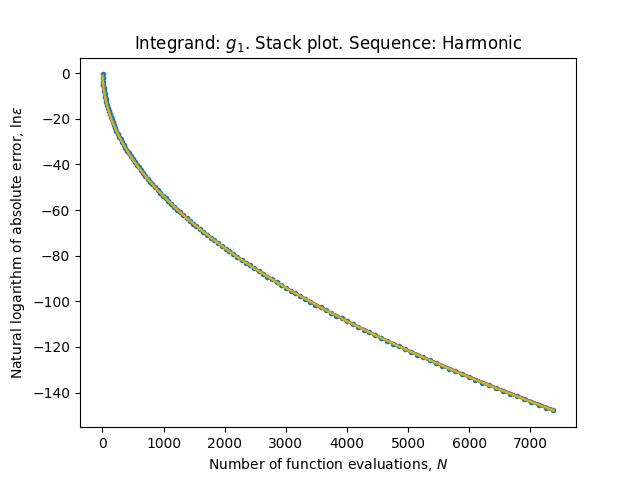
\includegraphics[scale=0.45]{../results/romberg_plots/g_one_hp_harmonic_stack.png}
\end{minipage}
\begin{minipage}{0.45\textwidth}
\centering
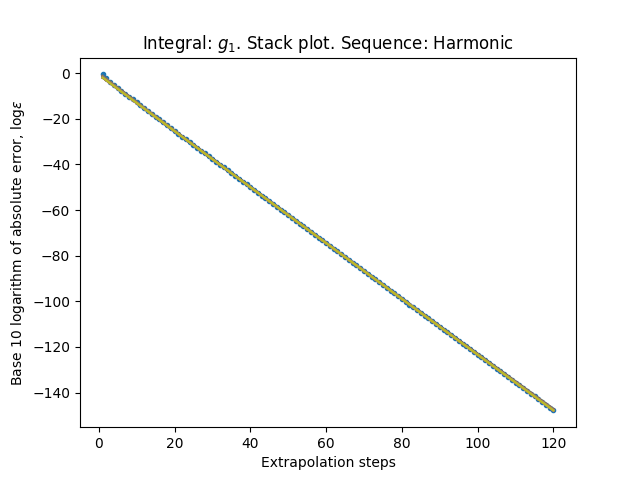
\includegraphics[scale=0.45]{../results/romberg_plots/g_one_hp_harmonic_steps_stack.png}
\end{minipage}
\end{figure}

\begin{figure}[H]
\centering
\begin{minipage}{0.45\textwidth}
\centering
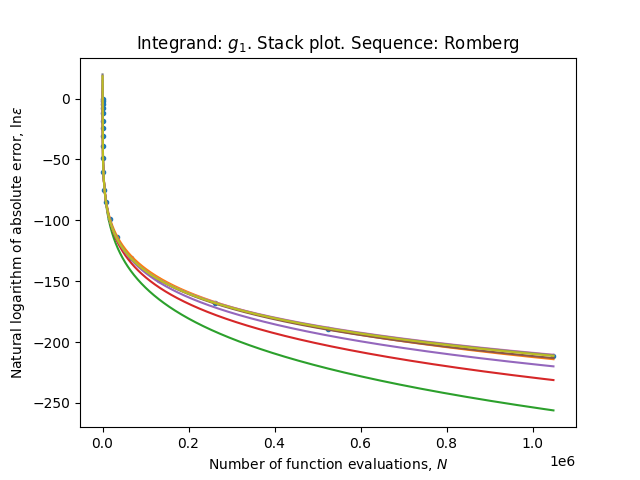
\includegraphics[scale=0.45]{../results/romberg_plots/g_one_hp_romberg_stack.png}
\end{minipage}
\begin{minipage}{0.45\textwidth}
\centering
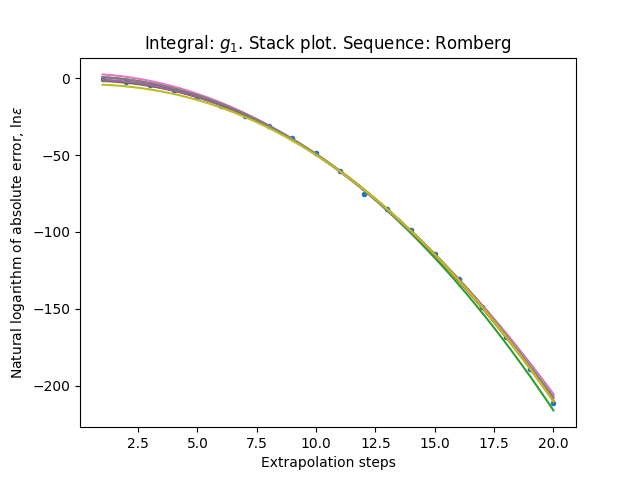
\includegraphics[scale=0.45]{../results/romberg_plots/g_one_hp_romberg_steps_stack.png}
\end{minipage}
\end{figure}

\begin{figure}[H]
\centering
\begin{minipage}{0.45\textwidth}
\centering
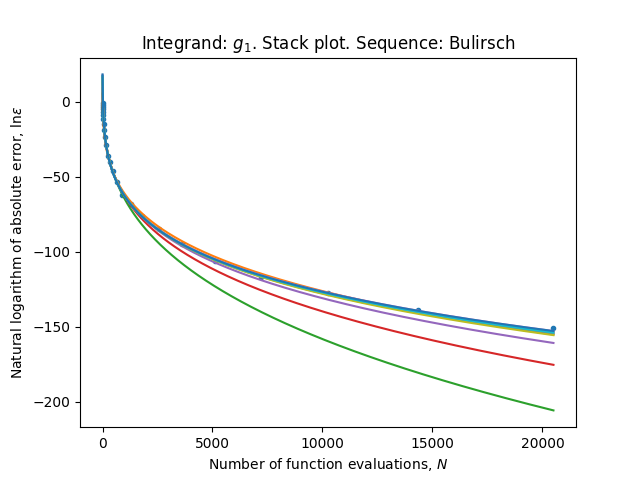
\includegraphics[scale=0.45]{../results/romberg_plots/g_one_hp_bulirsch_stack.png}
\end{minipage}
\begin{minipage}{0.45\textwidth}
\centering
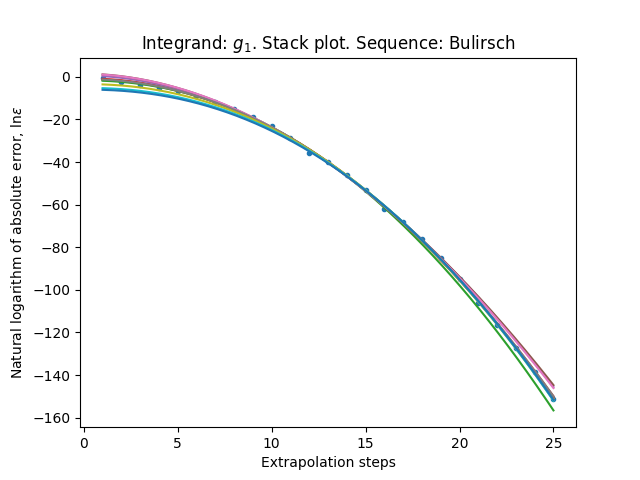
\includegraphics[scale=0.45]{../results/romberg_plots/g_one_hp_bulirsch_steps_stack.png}
\end{minipage}
\end{figure}

\begin{table}[H]
    \centering
        \small
        \begin{tabular}{c||c|c|c|c|c|c|c|c}
Sequence & \(A\)-mean & \(A\)-var & \(c\)-mean & \(c\)-var & \(q\)-mean & \(q\)-var & \(\rho_{\operatorname{lin}}\) & \(\rho_{\ln}\)\\\hline
\rowcolor{green}
Harmonic & \(3.771\) & \(0.02895\) & \(1.793\) & \(0.0001375\) & \(0.4963\) & \(6.495\cdot 10^{-6}\) & \(0.1014\) & \(3.209\cdot 10^{-7}\) \\
\rowcolor{yellow}
Romberg & \(4.114\cdot 10^{37}\) & \(5.211\) & \(46.94\) & \(0.1026\) & \(0.135\) & \(0.03489\) & \(1.548\cdot 10^5\) & \(0.0005732\) \\
\rowcolor{yellow}
Bulirsch & \(8.199\cdot 10^{22}\) & \(4.987\) & \(24.22\) & \(0.1103\) & \(0.2236\) & \(0.04529\) & \(3.921\cdot 10^5\) & \(0.001355\) \\
\rowcolor{green}
Harmonic & \(0.6596\) & \(0.04548\) & \(1.277\) & \(0.0002625\) & \(0.9918\) & \(1.093\cdot 10^{-5}\) & \(0.2565\) & \(1.067\cdot 10^{-6}\) \\
\rowcolor{red}
Romberg & \(3.747\) & \(2.921\) & \(0.4181\) & \(0.02976\) & \(2.079\) & \(0.0008172\) & \(0.2401\) & \(7.665\cdot 10^{-5}\) \\
\rowcolor{red}
Bulirsch & \(1.191\) & \(1.72\) & \(0.2048\) & \(0.105\) & \(2.062\) & \(0.00252\) & \(0.3619\) & \(9.058\cdot 10^{-5}\) \\
    \end{tabular}
    \label{tab:my_label}
\end{table}

We see that the harmonic sequence performes best, then Bulirsch and then Romberg. In standard double precision arithmetic, we get down to machine level precision using Romberg or Bulirsch, but we are like \(5\) digits from there, using the harmonic sequence.\\

Here we clearly have exponential convergence in the number of evaluations for the Harmonic sequence and hence also in the number of steps. We do not have exponential convergence in the number of evaluations for Romberg and Bulirsch but the model for exponential convergence in the number of steps fits moderately well for those sequences. 

\subsubsection{\(a = 10^{-1}\)}

\begin{figure}[H]
\centering
\begin{minipage}{0.45\textwidth}
\centering
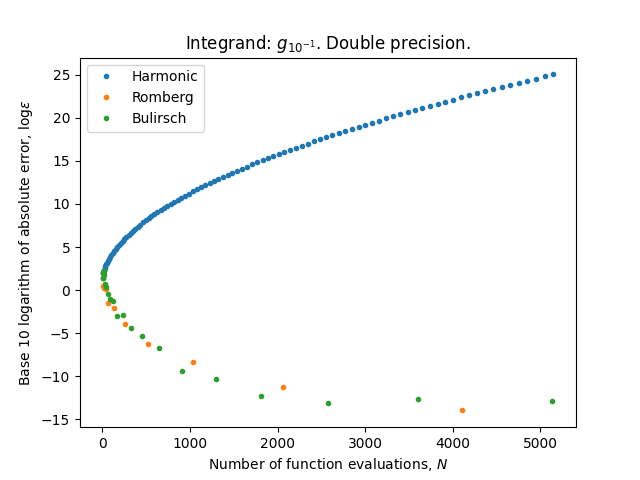
\includegraphics[scale=0.45]{../results/romberg_plots/g_tenth.png}
\end{minipage}
\begin{minipage}{0.45\textwidth}
\centering
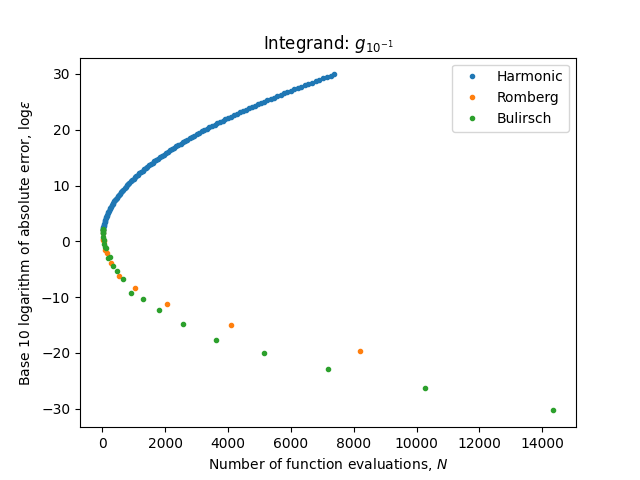
\includegraphics[scale=0.45]{../results/romberg_plots/g_tenth_hp.png}
\end{minipage}
\end{figure}

\begin{figure}[H]
\centering
\begin{minipage}{0.45\textwidth}
\centering
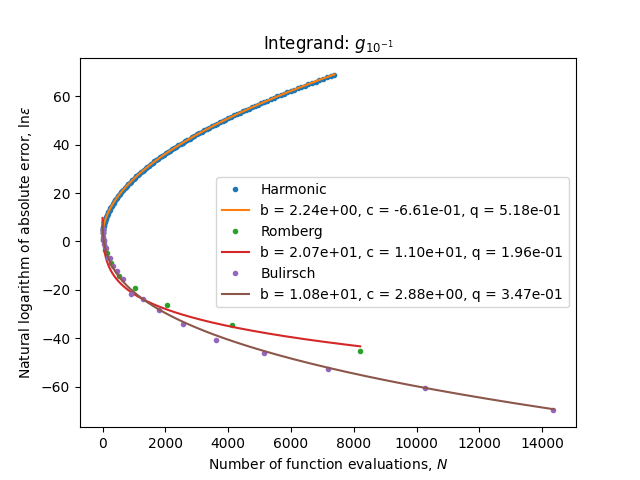
\includegraphics[scale=0.45]{../results/romberg_plots/g_tenth_hp_trend.png}
\end{minipage}
\begin{minipage}{0.45\textwidth}
\centering
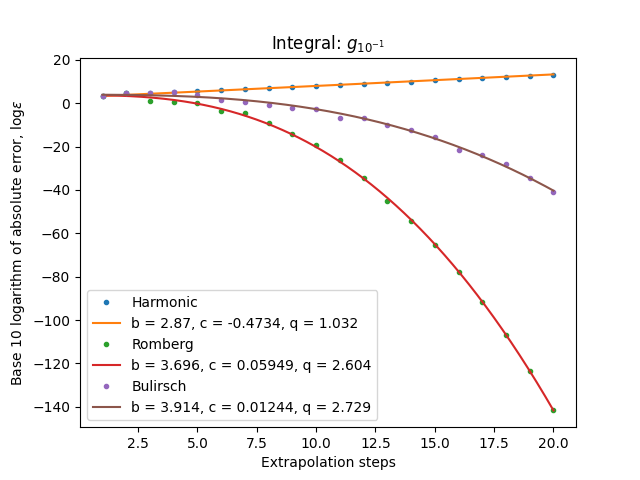
\includegraphics[scale=0.45]{../results/romberg_plots/g_tenth_hp_steps.png}
\end{minipage}
\end{figure}

\begin{figure}[H]
\centering
\begin{minipage}{0.45\textwidth}
\centering
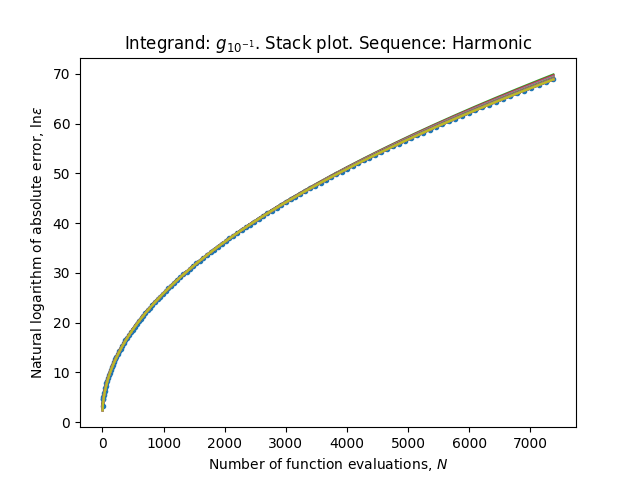
\includegraphics[scale=0.45]{../results/romberg_plots/g_tenth_hp_harmonic_stack.png}
\end{minipage}
\begin{minipage}{0.45\textwidth}
\centering
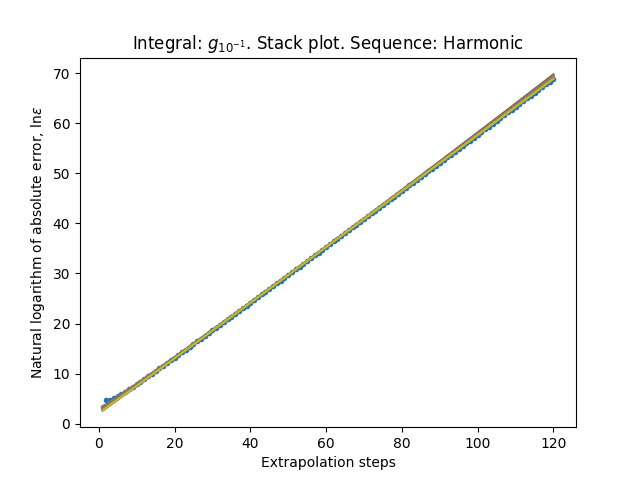
\includegraphics[scale=0.45]{../results/romberg_plots/g_tenth_hp_harmonic_steps_stack.png}
\end{minipage}
\end{figure}

\begin{figure}[H]
\centering
\begin{minipage}{0.45\textwidth}
\centering
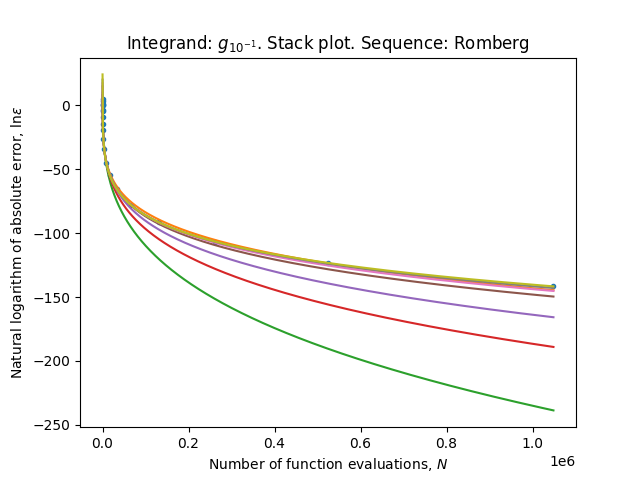
\includegraphics[scale=0.45]{../results/romberg_plots/g_tenth_hp_romberg_stack.png}
\end{minipage}
\begin{minipage}{0.45\textwidth}
\centering
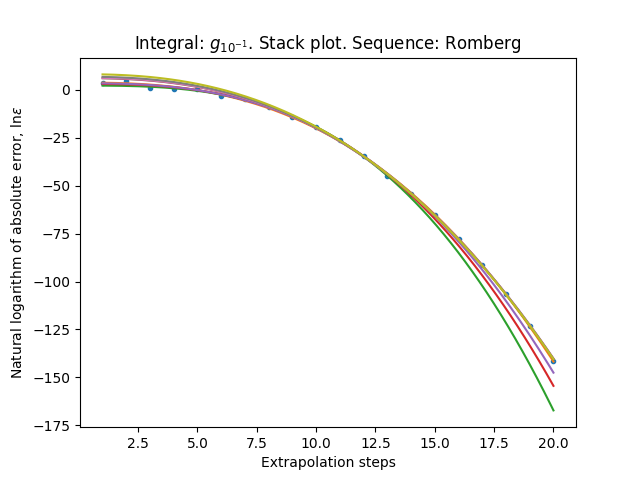
\includegraphics[scale=0.45]{../results/romberg_plots/g_tenth_hp_romberg_steps_stack.png}
\end{minipage}
\end{figure}

\begin{figure}[H]
\centering
\begin{minipage}{0.45\textwidth}
\centering
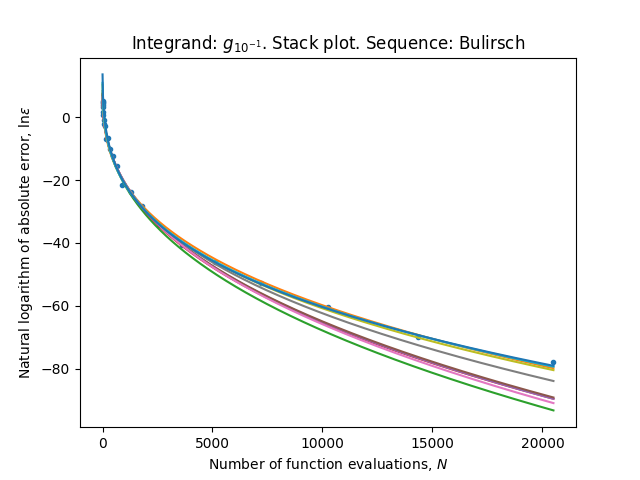
\includegraphics[scale=0.45]{../results/romberg_plots/g_tenth_hp_bulirsch_stack.png}
\end{minipage}
\begin{minipage}{0.45\textwidth}
\centering
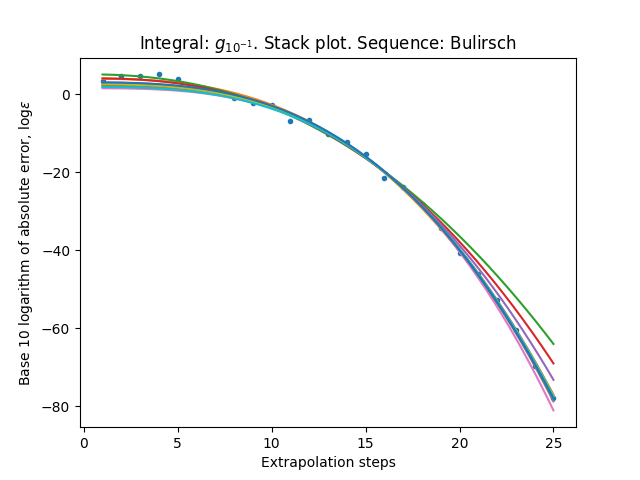
\includegraphics[scale=0.45]{../results/romberg_plots/g_tenth_hp_bulirsch_steps_stack.png}
\end{minipage}
\end{figure}

\begin{table}[H]
    \centering
        \small
    \begin{tabular}{c||c|c|c|c|c|c|c|c}
Sequence & \(A\)-mean & \(A\)-var & \(c\)-mean & \(c\)-var & \(q\)-mean & \(q\)-var & \(\rho_{\operatorname{lin}}\) & \(\rho_{\ln}\)\\\hline
\rowcolor{red}
Harmonic & \(5.231\) & \(0.0773\) & \(-0.7178\) & \(0.001803\) & \(0.5101\) & \(9.026\cdot 10^{-5}\) & \(0.01647\) & \(8.663\cdot 10^{-6}\) \\
\rowcolor{red}
Romberg & \(7.533\cdot 10^{22}\) & \(5.999\) & \(14.35\) & \(0.3322\) & \(0.2047\) & \(0.07855\) & \(974.3\) & \(0.001405\) \\
\rowcolor{red}
Bulirsch & \(8.963\cdot 10^7\) & \(7.604\) & \(2.995\) & \(0.186\) & \(0.3602\) & \(0.0129\) & \(33.54\) & \(0.001672\) \\
\rowcolor{red}
Harmonic & \(10.97\) & \(0.05032\) & \(-0.5086\) & \(0.001492\) & \(1.019\) & \(6.47\cdot 10^{-5}\) & \(0.01168\) & \(6.684\cdot 10^{-6}\) \\
\rowcolor{yellow}
Romberg & \(727.7\) & \(2.108\) & \(0.06624\) & \(0.1819\) & \(2.623\) & \(0.005292\) & \(0.521\) & \(0.0001729\) \\
\rowcolor{yellow}
Bulirsch & \(32.46\) & \(2.026\) & \(0.01381\) & \(0.7483\) & \(2.764\) & \(0.006506\) & \(0.5118\) & \(0.0008637\) \\
    \end{tabular}
    \label{tab:my_label}
\end{table}

Here we get divergence for the harmonic sequence, but convergence for the other sequences, fastest for Bulirsch. In standard double precision arithmetic, we get down to machine level precision using Romberg or Bulirsch. The model for exponential convergence in number of evaluations does not fit for Bulirsch nor Romberg but it is hard to tell whether we have exponential convergence in the number of steps.

\subsubsection{\(a = 10^{-2}\)}

\begin{figure}[H]
\centering
\begin{minipage}{0.45\textwidth}
\centering
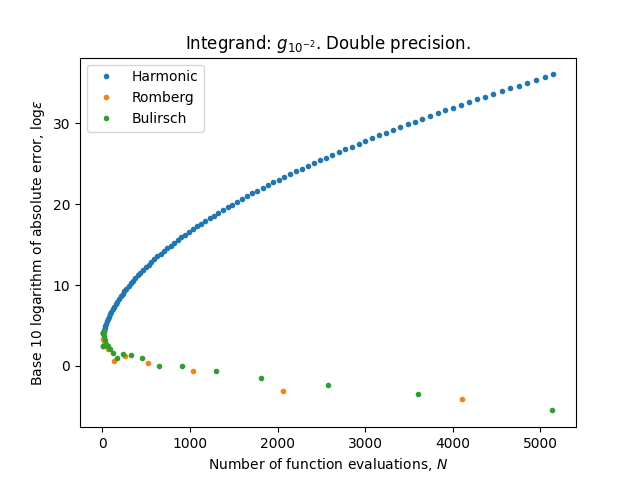
\includegraphics[scale=0.45]{../results/romberg_plots/g_hundredth.png}
\end{minipage}
\begin{minipage}{0.45\textwidth}
\centering
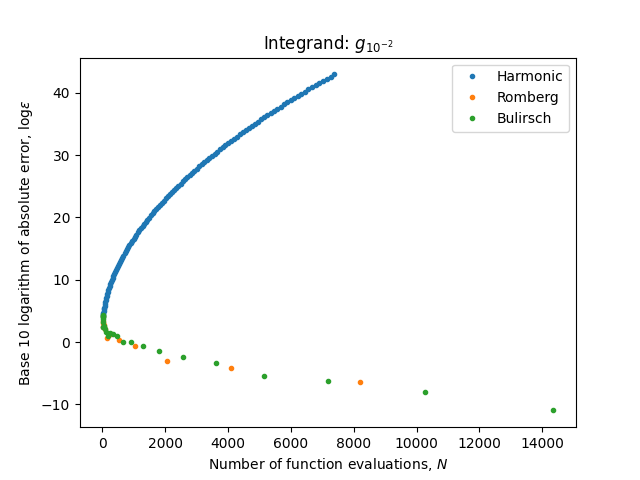
\includegraphics[scale=0.45]{../results/romberg_plots/g_hundredth_hp.png}
\end{minipage}
\end{figure}

\begin{figure}[H]
\centering
\begin{minipage}{0.45\textwidth}
\centering
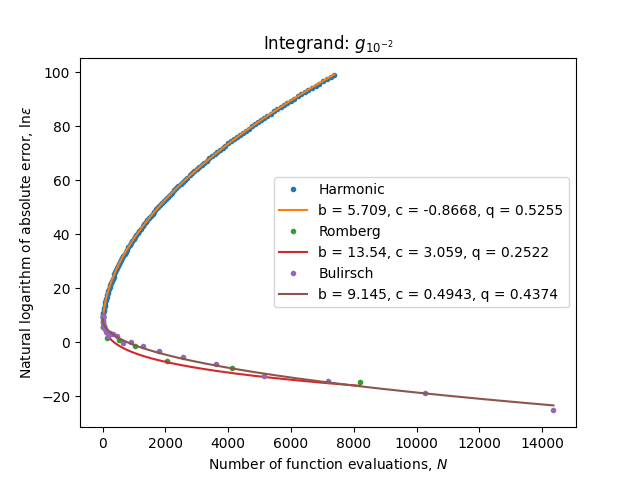
\includegraphics[scale=0.45]{../results/romberg_plots/g_hundredth_hp_trend.png}
\end{minipage}
\begin{minipage}{0.45\textwidth}
\centering
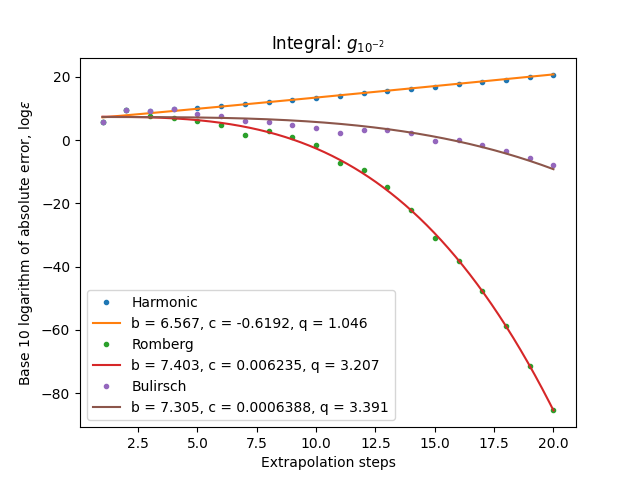
\includegraphics[scale=0.45]{../results/romberg_plots/g_hundredth_hp_steps.png}
\end{minipage}
\end{figure}

\begin{figure}[H]
\centering
\begin{minipage}{0.45\textwidth}
\centering
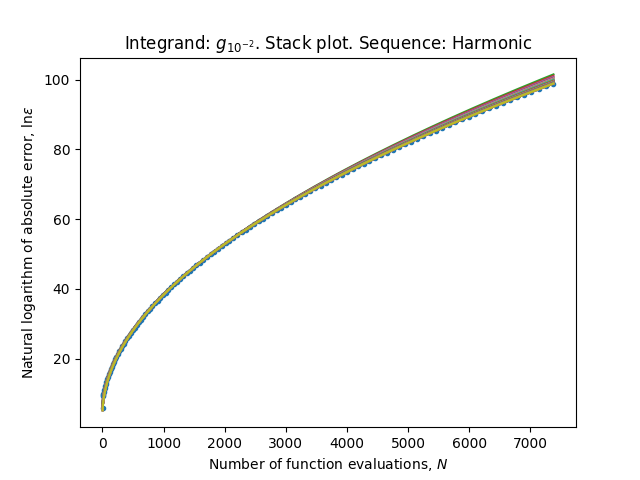
\includegraphics[scale=0.45]{../results/romberg_plots/g_hundredth_hp_harmonic_stack.png}
\end{minipage}
\begin{minipage}{0.45\textwidth}
\centering
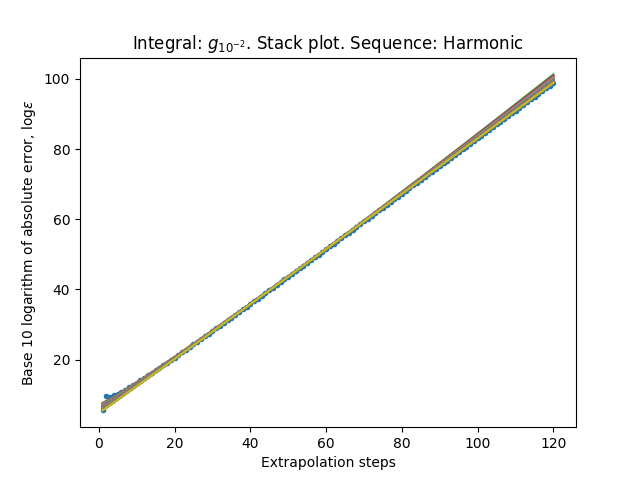
\includegraphics[scale=0.45]{../results/romberg_plots/g_hundredth_hp_harmonic_steps_stack.png}
\end{minipage}
\end{figure}

\begin{figure}[H]
\centering
\begin{minipage}{0.45\textwidth}
\centering
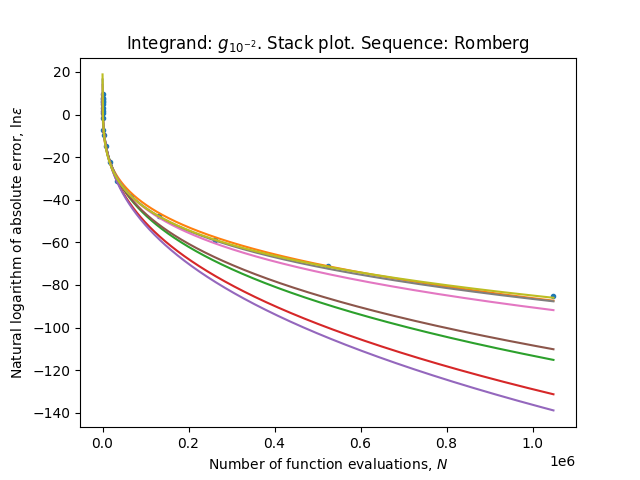
\includegraphics[scale=0.45]{../results/romberg_plots/g_hundredth_hp_romberg_stack.png}
\end{minipage}
\begin{minipage}{0.45\textwidth}
\centering
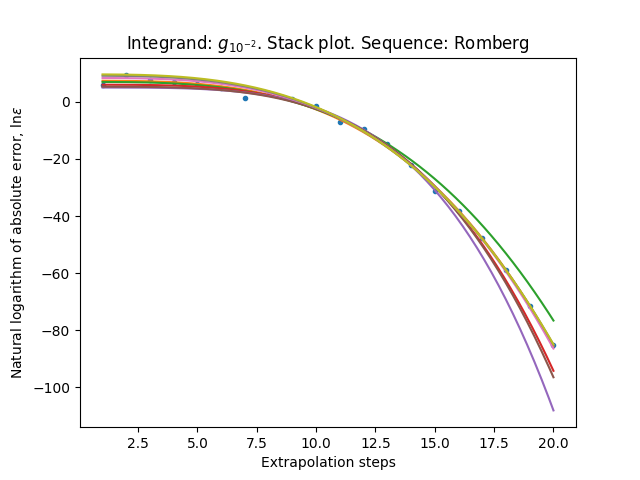
\includegraphics[scale=0.45]{../results/romberg_plots/g_hundredth_hp_romberg_steps_stack.png}
\end{minipage}
\end{figure}

\begin{figure}[H]
\centering
\begin{minipage}{0.45\textwidth}
\centering
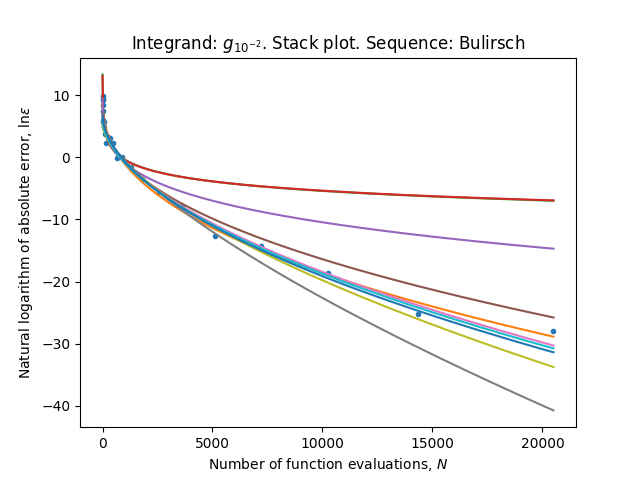
\includegraphics[scale=0.45]{../results/romberg_plots/g_hundredth_hp_bulirsch_stack.png}
\end{minipage}
\begin{minipage}{0.45\textwidth}
\centering
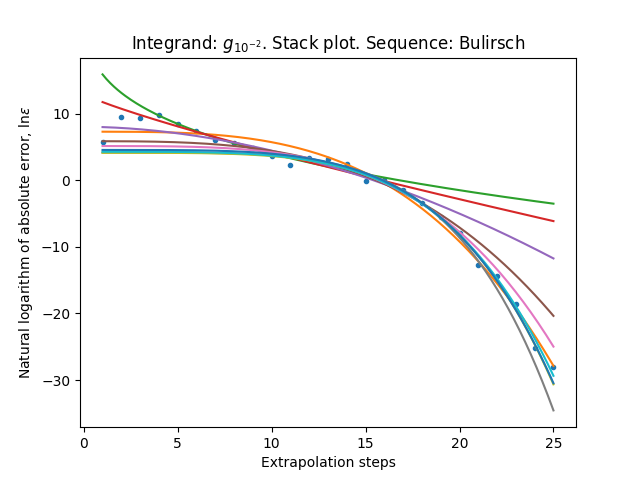
\includegraphics[scale=0.45]{../results/romberg_plots/g_hundredth_hp_bulirsch_steps_stack.png}
\end{minipage}
\end{figure}

\begin{table}[H]
    \centering
    \small
    \begin{tabular}{c||c|c|c|c|c|c|c|c}
Sequence & \(A\)-mean & \(A\)-var & \(c\)-mean & \(c\)-var & \(q\)-mean & \(q\)-var & \(\rho_{\operatorname{lin}}\) & \(\rho_{\ln}\)\\\hline
\rowcolor{red}
Harmonic & \(122.7\) & \(0.8001\) & \(-0.9641\) & \(0.007205\) & \(0.5155\) & \(0.0003682\) & \(0.07171\) & \(1.955\cdot 10^{-5}\) \\
\rowcolor{red}
Romberg & \(8.898\cdot 10^{10}\) & \(5.785\) & \(3.021\) & \(0.6343\) & \(0.2928\) & \(0.05447\) & \(2.317\) & \(0.00266\) \\
\rowcolor{red}
Bulirsch & \(\cdot\) & \(\cdot\) & \(2876\) & \(4.874\) & \(0.4042\) & \(0.3708\) & \(0.7208\) & \(0.01268\) \\
\rowcolor{red}
Harmonic & \(323.1\) & \(0.5753\) & \(-0.682\) & \(0.006766\) & \(1.029\) & \(0.0002999\) & \(0.05485\) & \(1.857\cdot 10^{-5}\) \\
\rowcolor{yellow}
Romberg & \(4384\) & \(1.505\) & \(0.005443\) & \(0.4455\) & \(3.388\) & \(0.0103\) & \(0.76\) & \(0.001069\) \\
\rowcolor{red}
Bulirsch & \(1.73\cdot 10^{11}\) & \(8\) & \(1.498\) & \(6.41\) & \(3.17\) & \(0.272\) & \(0.8139\) & \(0.01705\) \\
    \end{tabular}
    \label{tab:my_label}
\end{table}

Here the same comments apply as for \(a = 10^{-1}\), except that now the Romberg sequence performes better than the Bulirsch sequence and the model fitting is worse. 

\subsection{Logarithm}

Now we will consider the following function 
\[
h_a: [0, 1] \rightarrow \R, \quad h_a(x) \coloneqq \ln(a + x),\, a > 0.
\]
This function is analytic on neighbourhood about the interval but we have a singularity at the horizontal ray from \(-a\) to \(-\infty\).

\subsubsection{\(a = 1\)}

\begin{figure}[H]
\centering
\begin{minipage}{0.45\textwidth}
\centering
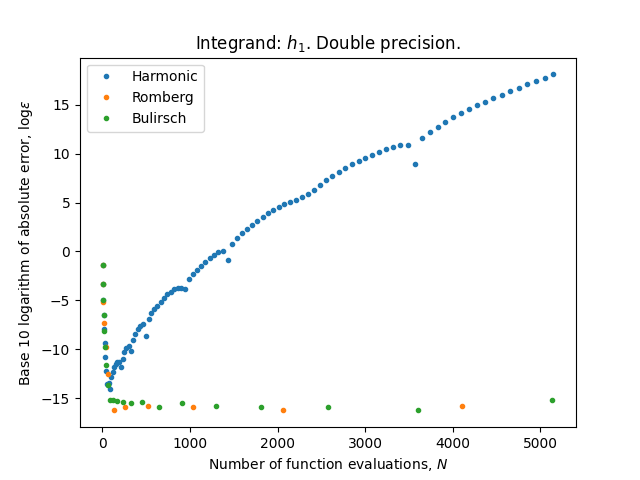
\includegraphics[scale=0.45]{../results/romberg_plots/h_one.png}
\end{minipage}
\begin{minipage}{0.45\textwidth}
\centering
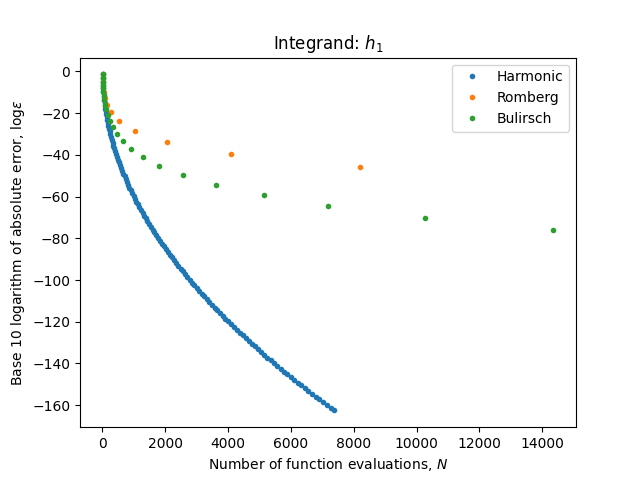
\includegraphics[scale=0.45]{../results/romberg_plots/h_one_hp.png}
\end{minipage}
\end{figure}

\begin{figure}[H]
\centering
\begin{minipage}{0.45\textwidth}
\centering
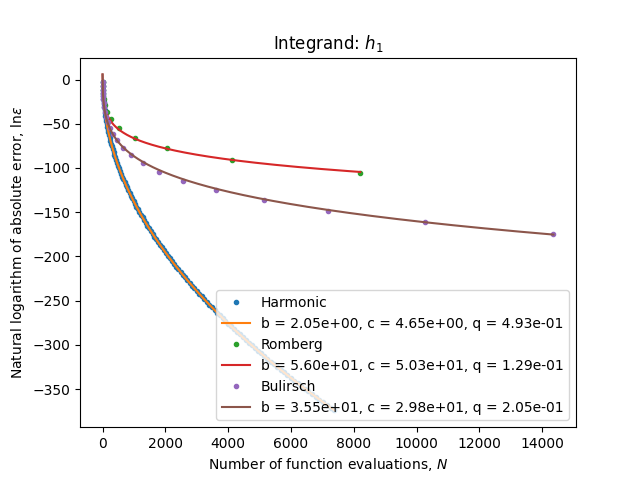
\includegraphics[scale=0.45]{../results/romberg_plots/h_one_hp_trend.png}
\end{minipage}
\begin{minipage}{0.45\textwidth}
\centering
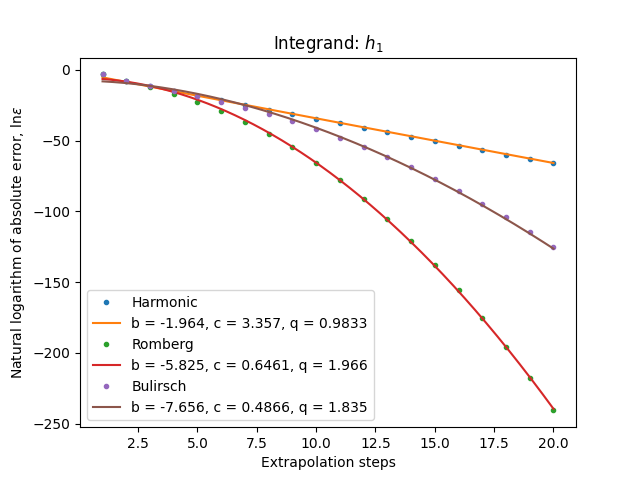
\includegraphics[scale=0.45]{../results/romberg_plots/h_one_hp_steps.png}
\end{minipage}
\end{figure}

\begin{figure}[H]
\centering
\begin{minipage}{0.45\textwidth}
\centering
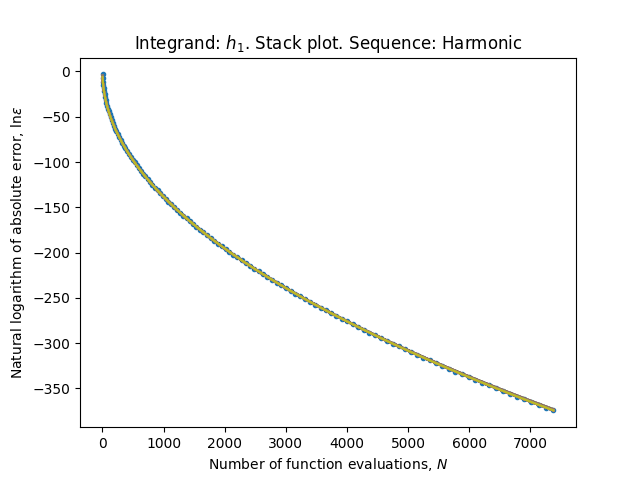
\includegraphics[scale=0.45]{../results/romberg_plots/h_one_hp_harmonic_stack.png}
\end{minipage}
\begin{minipage}{0.45\textwidth}
\centering
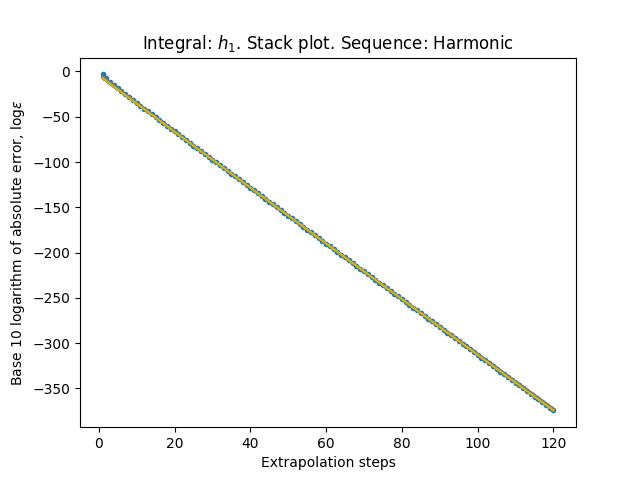
\includegraphics[scale=0.45]{../results/romberg_plots/h_one_hp_harmonic_steps_stack.png}
\end{minipage}
\end{figure}

\begin{figure}[H]
\centering
\begin{minipage}{0.45\textwidth}
\centering
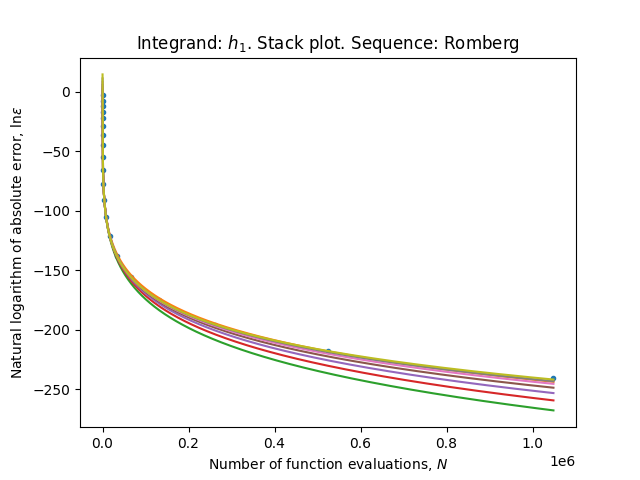
\includegraphics[scale=0.45]{../results/romberg_plots/h_one_hp_romberg_stack.png}
\end{minipage}
\begin{minipage}{0.45\textwidth}
\centering
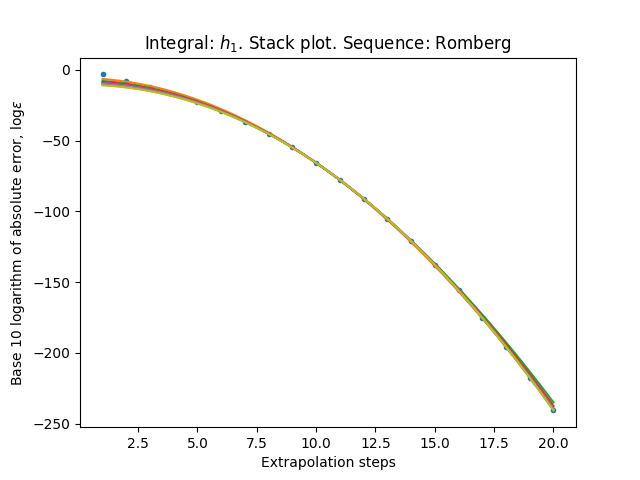
\includegraphics[scale=0.45]{../results/romberg_plots/h_one_hp_romberg_steps_stack.png}
\end{minipage}
\end{figure}

\begin{figure}[H]
\centering
\begin{minipage}{0.45\textwidth}
\centering
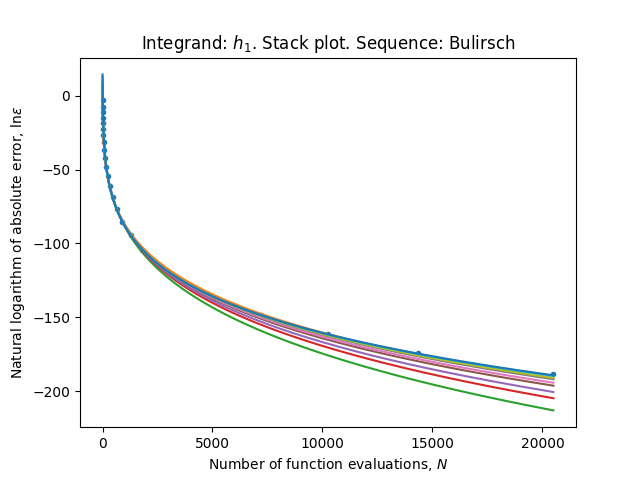
\includegraphics[scale=0.45]{../results/romberg_plots/h_one_hp_bulirsch_stack.png}
\end{minipage}
\begin{minipage}{0.45\textwidth}
\centering
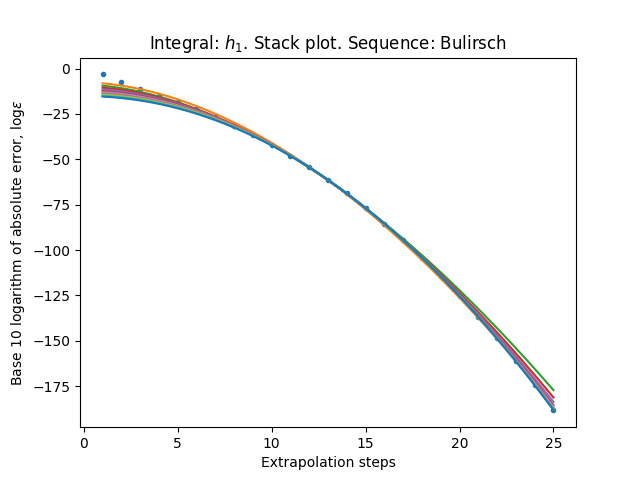
\includegraphics[scale=0.45]{../results/romberg_plots/h_one_hp_bulirsch_steps_stack.png}
\end{minipage}
\end{figure}

\begin{table}[H]
    \centering
    \small
    \begin{tabular}{c||c|c|c|c|c|c|c|c}
Sequence & \(A\)-mean & \(A\)-var & \(c\)-mean & \(c\)-var & \(q\)-mean & \(q\)-var & \(\rho_{\operatorname{lin}}\) & \(\rho_{\ln}\)\\\hline
\rowcolor{green}
Harmonic & \(3.072\) & \(0.3632\) & \(4.545\) & \(0.000229\) & \(0.4954\) & \(1.085\cdot 10^{-5}\) & \(0.5183\) & \(6.335\cdot 10^{-7}\) \\
\rowcolor{red}
Romberg & \(1.538\cdot 10^{43}\) & \(6\) & \(56.82\) & \(0.06603\) & \(0.1269\) & \(0.0163\) & \(4054\) & \(0.0002381\) \\
\rowcolor{red}
Bulirsch & \(1.55\cdot 10^{31}\) & \(7.894\) & \(36.84\) & \(0.08131\) & \(0.1955\) & \(0.0187\) & \(7380\) & \(0.0003219\) \\
\rowcolor{green}
Harmonic & \(0.03919\) & \(0.5477\) & \(3.237\) & \(0.0003865\) & \(0.9901\) & \(1.608\cdot 10^{-5}\) & \(0.7691\) & \(1.584\cdot 10^{-6}\) \\
\rowcolor{yellow}
Romberg & \(0.0002063\) & \(1.214\) & \(0.5431\) & \(0.009515\) & \(2.02\) & \(0.000263\) & \(0.9235\) & \(7.907\cdot 10^{-5}\) \\
\rowcolor{yellow}
Bulirsch & \(2.293\cdot 10^{-5}\) & \(3.407\) & \(0.3579\) & \(0.06839\) & \(1.929\) & \(0.001656\) & \(0.9854\) & \(0.0002632\) \\
    \end{tabular}
    \label{tab:my_label}
\end{table}

We see that the harmonic sequence performes best, then Bulirsch and then Romberg. In standard double precision arithmetic, we get down to machine level precision using Romberg or Bulirsch, but we are like \(2\) digits from there, using the harmonic sequence.\\

Here we clearly have exponential convergence in the number of evaluations for the harmonic sequence and hence also in the number of steps. For Romberg and Bulirsch we seem to have exponential convergence in the number of steps though the fitting is not as nice as in the case of the harmonic sequence.

\subsubsection{\(a= 10^{-2}\)}

\begin{figure}[H]
\centering
\begin{minipage}{0.45\textwidth}
\centering
\includegraphics[scale=0.45]{../results/romberg_plots/h_hundredth.png}
\end{minipage}
\begin{minipage}{0.45\textwidth}
\centering
\includegraphics[scale=0.45]{../results/romberg_plots/h_hundredth_hp.png}
\end{minipage}
\end{figure}

\begin{figure}[H]
\centering
\begin{minipage}{0.45\textwidth}
\centering
\includegraphics[scale=0.45]{../results/romberg_plots/h_hundredth_hp_trend.png}
\end{minipage}
\begin{minipage}{0.45\textwidth}
\centering
\includegraphics[scale=0.45]{../results/romberg_plots/h_hundredth_hp_steps.png}
\end{minipage}
\end{figure}

\begin{figure}[H]
\centering
\begin{minipage}{0.45\textwidth}
\centering
\includegraphics[scale=0.45]{../results/romberg_plots/h_hundredth_hp_harmonic_stack.png}
\end{minipage}
\begin{minipage}{0.45\textwidth}
\centering
\includegraphics[scale=0.45]{../results/romberg_plots/h_hundredth_hp_harmonic_steps_stack.png}
\end{minipage}
\end{figure}

\begin{figure}[H]
\centering
\begin{minipage}{0.45\textwidth}
\centering
\includegraphics[scale=0.45]{../results/romberg_plots/h_hundredth_hp_romberg_stack.png}
\end{minipage}
\begin{minipage}{0.45\textwidth}
\centering
\includegraphics[scale=0.45]{../results/romberg_plots/h_hundredth_hp_romberg_steps_stack.png}
\end{minipage}
\end{figure}

\begin{figure}[H]
\centering
\begin{minipage}{0.45\textwidth}
\centering
\includegraphics[scale=0.45]{../results/romberg_plots/h_hundredth_hp_bulirsch_stack.png}
\end{minipage}
\begin{minipage}{0.45\textwidth}
\centering
\includegraphics[scale=0.45]{../results/romberg_plots/h_hundredth_hp_bulirsch_steps_stack.png}
\end{minipage}
\end{figure}

\begin{table}[H]
    \centering
    \small
    \begin{tabular}{c||c|c|c|c|c|c|c|c}
Sequence & \(A\)-mean & \(A\)-var & \(c\)-mean & \(c\)-var & \(q\)-mean & \(q\)-var & \(\rho_{\operatorname{lin}}\) & \(\rho_{\ln}\)\\\hline
\rowcolor{yellow}
Harmonic & \(0.1351\) & \(2.455\) & \(0.6631\) & \(0.1084\) & \(0.4296\) & \(0.004684\) & \(0.7131\) & \(0.0001955\) \\
\rowcolor{red}
Romberg & \(3.388\cdot 10^9\) & \(5.969\) & \(6.696\) & \(0.2315\) & \(0.2286\) & \(0.02614\) & \(7.917\) & \(0.0005581\) \\
\rowcolor{yellow}
Bulirsch & \(6.859\) & \(1.956\) & \(1.626\) & \(0.0311\) & \(0.3675\) & \(0.002076\) & \(0.2014\) & \(0.0001172\) \\
\rowcolor{yellow}
Harmonic & \(0.07535\) & \(1.798\) & \(0.4822\) & \(0.1106\) & \(0.8628\) & \(0.0042\) & \(0.7117\) & \(0.0001939\) \\
\rowcolor{yellow}
Romberg & \(0.05205\) & \(0.2618\) & \(0.02252\) & \(0.01836\) & \(2.848\) & \(0.0002742\) & \(0.7571\) & \(0.0001742\) \\
\rowcolor{red}
Bulirsch & \(0.0214\) & \(1.016\) & \(0.00882\) & \(1.141\) & \(2.822\) & \(0.01164\) & \(0.8803\) & \(0.00138\) \\
    \end{tabular}
    \label{tab:my_label}
\end{table}

We see that we can not attain high precision using the harmonic sequence and standard double precision. It is hard to tell which sequence performes best in the long run, though we can say that Bulirsch performes better than Romberg.\\

For Romberg, we get a moderately goot fit for exponential convergence in the number of steps. The fitting is quite good for the harmonic sequence but it is quite unstable for Bulirsch.

\subsubsection{\(a = 10^{-4}\)}

\begin{figure}[H]
\centering
\begin{minipage}{0.45\textwidth}
\centering
\includegraphics[scale=0.45]{../results/romberg_plots/h_tenthousandth.png}
\end{minipage}
\begin{minipage}{0.45\textwidth}
\centering
\includegraphics[scale=0.45]{../results/romberg_plots/h_tenthousandth_hp.png}
\end{minipage}
\end{figure}

\begin{figure}[H]
\centering
\begin{minipage}{0.45\textwidth}
\centering
\includegraphics[scale=0.45]{../results/romberg_plots/h_tenthousandth_hp_trend.png}
\end{minipage}
\begin{minipage}{0.45\textwidth}
\centering
\includegraphics[scale=0.45]{../results/romberg_plots/h_tenthousandth_hp_steps.png}
\end{minipage}
\end{figure}

\begin{figure}[H]
\centering
\begin{minipage}{0.45\textwidth}
\centering
\includegraphics[scale=0.45]{../results/romberg_plots/h_tenthousandth_hp_harmonic_stack.png}
\end{minipage}
\begin{minipage}{0.45\textwidth}
\centering
\includegraphics[scale=0.45]{../results/romberg_plots/h_tenthousandth_hp_harmonic_steps_stack.png}
\end{minipage}
\end{figure}

\begin{figure}[H]
\centering
\begin{minipage}{0.45\textwidth}
\centering
\includegraphics[scale=0.45]{../results/romberg_plots/h_tenthousandth_hp_romberg_stack.png}
\end{minipage}
\begin{minipage}{0.45\textwidth}
\centering
\includegraphics[scale=0.45]{../results/romberg_plots/h_tenthousandth_hp_romberg_steps_stack.png}
\end{minipage}
\end{figure}

\begin{figure}[H]
\centering
\begin{minipage}{0.45\textwidth}
\centering
\includegraphics[scale=0.45]{../results/romberg_plots/h_tenthousandth_hp_bulirsch_stack.png}
\end{minipage}
\begin{minipage}{0.45\textwidth}
\centering
\includegraphics[scale=0.45]{../results/romberg_plots/h_tenthousandth_hp_bulirsch_steps_stack.png}
\end{minipage}
\end{figure}

\begin{table}[H]
    \centering
    \small
    \begin{tabular}{c||c|c|c|c|c|c|c|c}
Sequence & \(A\)-mean & \(A\)-var & \(c\)-mean & \(c\)-var & \(q\)-mean & \(q\)-var & \(\rho_{\operatorname{lin}}\) & \(\rho_{\ln}\)\\\hline
\rowcolor{yellow}
Harmonic & \(1.328\cdot 10^{13}\) & \(55.82\) & \(8.14\) & \(0.5474\) & \(0.09568\) & \(0.0936\) & \(0.1034\) & \(9.631\cdot 10^{-5}\) \\
\rowcolor{red}
Romberg & \(106.1\) & \(5.445\) & \(2.037\) & \(0.7267\) & \(0.2364\) & \(0.06414\) & \(0.6139\) & \(0.001346\) \\
\rowcolor{red}
Bulirsch & \(1.888\cdot 10^5\) & \(5.399\) & \(6.394\) & \(0.3315\) & \(0.1362\) & \(0.1274\) & \(0.1687\) & \(0.0008794\) \\
\rowcolor{yellow}
Harmonic & \(1.395\cdot 10^4\) & \(17.13\) & \(5.261\) & \(0.2049\) & \(0.2157\) & \(0.04738\) & \(0.04431\) & \(4.038\cdot 10^{-5}\) \\
\rowcolor{red}
Romberg & \(0.1362\) & \(2.091\) & \(0.02426\) & \(2.55\) & \(3.039\) & \(0.07013\) & \(0.8591\) & \(0.004444\) \\
\rowcolor{red}
Bulirsch & \(0.4121\) & \(0.6973\) & \(0.09479\) & \(0.8435\) & \(1.695\) & \(0.05417\) & \(0.4717\) & \(0.003557\) \\
    \end{tabular}
    \label{tab:my_label}
\end{table}

Here again, we do not attain high precision when using the Harmonic sequence in double precision arithmetic. It is hard to say which sequence performes best. We get reasonably good fit for the harmonic sequence but not for Romberg and Bulirsch.

\subsection{Area of half circle}

Now we will try the following function:
\[
i: [-1, 1] \rightarrow \R, \quad i(x)\coloneqq \sqrt{1-x^2}.
\]
This function is analytic inside the interval of definition but not at the endpoints. Its derivative has singularities at the endpoints.

\begin{figure}[H]
\centering
\begin{minipage}{0.45\textwidth}
\centering
\includegraphics[scale=0.45]{../results/romberg_plots/circle_area.png}
\end{minipage}
\begin{minipage}{0.45\textwidth}
\centering
\includegraphics[scale=0.45]{../results/romberg_plots/circle_area_hp.png}
\end{minipage}
\end{figure}

\begin{figure}[H]
\centering
\begin{minipage}{0.45\textwidth}
\centering
\includegraphics[scale=0.45]{../results/romberg_plots/circle_area_hp_trend.png}
\end{minipage}
\begin{minipage}{0.45\textwidth}
\centering
\includegraphics[scale=0.45]{../results/romberg_plots/circle_area_hp_steps.png}
\end{minipage}
\end{figure}

\begin{figure}[H]
\centering
\begin{minipage}{0.45\textwidth}
\centering
\includegraphics[scale=0.45]{../results/romberg_plots/circle_area_hp_harmonic_stack.png}
\end{minipage}
\begin{minipage}{0.45\textwidth}
\centering
\includegraphics[scale=0.45]{../results/romberg_plots/circle_area_hp_harmonic_steps_stack.png}
\end{minipage}
\end{figure}

\begin{figure}[H]
\centering
\begin{minipage}{0.45\textwidth}
\centering
\includegraphics[scale=0.45]{../results/romberg_plots/circle_area_hp_romberg_stack.png}
\end{minipage}
\begin{minipage}{0.45\textwidth}
\centering
\includegraphics[scale=0.45]{../results/romberg_plots/circle_area_hp_romberg_steps_stack.png}
\end{minipage}
\end{figure}

\begin{figure}[H]
\centering
\begin{minipage}{0.45\textwidth}
\centering
\includegraphics[scale=0.45]{../results/romberg_plots/circle_area_hp_bulirsch_stack.png}
\end{minipage}
\begin{minipage}{0.45\textwidth}
\centering
\includegraphics[scale=0.45]{../results/romberg_plots/circle_area_hp_bulirsch_steps_stack.png}
\end{minipage}
\end{figure}

\begin{table}[H]
    \centering
    \small
    \begin{tabular}{c||c|c|c|c|c|c|c|c}
Sequence & \(A\)-mean & \(A\)-var & \(c\)-mean & \(c\)-var & \(q\)-mean & \(q\)-var & \(\rho_{\operatorname{lin}}\) & \(\rho_{\ln}\)\\\hline
\rowcolor{red}
Harmonic & \(\cdot\) & \(\cdot\) & \(5.358\cdot 10^4\) & \(0.003851\) & \(2.176\cdot 10^{-5}\) & \(0.00346\) & \(\cdot\) & \(0.0002451\) \\
\rowcolor{red}
Romberg & \(\cdot\) & \(\cdot\) & \(7.348\cdot 10^4\) & \(0.005727\) & \(2.071\cdot 10^{-5}\) & \(0.005124\) & \(\cdot\) & \(0.0002178\) \\
\rowcolor{red}
Bulirsch & \(\cdot\) & \(\cdot\) & \(5.763\cdot 10^4\) & \(0.0003158\) & \(2.647\cdot 10^{-5}\) & \(0.0002409\) & \(\cdot\) & \(0.0001299\) \\
\rowcolor{red}
Harmonic & \(\cdot\) & \(\cdot\) & \(6.694\cdot 10^4\) & \(0.0002388\) & \(3.364\cdot 10^{-5}\) & \(0.0002515\) & \(\cdot\) & \(1.351\cdot 10^{-5}\) \\
\rowcolor{green}
Romberg & \(1.581\) & \(0.0005141\) & \(1.046\) & \(5.395\cdot 10^{-5}\) & \(0.9983\) & \(4.956\cdot 10^{-6}\) & \(0.1245\) & \(0.0001394\) \\
\rowcolor{green}
Bulirsch & \(0.375\) & \(0.03054\) & \(0.5595\) & \(0.00836\) & \(0.9807\) & \(0.000633\) & \(0.2822\) & \(0.0007036\) \\
    \end{tabular}
    \label{tab:my_label}
\end{table}

We see that we do not get high precision using double precision arithmetic, independent of sequence. The Romberg and Bulirsch sequence seem to perform similarly well but the harmonic sequence seems to be slowest.\\

For the harmonic sequence we reject the fitting because we get unreasoable values of the parameters. The model for exponential convergence in the number of steps fits well in the case of the Romberg sequence and Bulirsch.

\subsection{Gaussian}

Finally we will consider the Gaussian function
\[
j: [0,1]\rightarrow \R, \quad k(x) \coloneqq \frac{2}{\sqrt{\pi}} e^{-x^2}.
\]
\begin{figure}[H]
\centering
\begin{minipage}{0.45\textwidth}
\centering
\includegraphics[scale=0.45]{../results/romberg_plots/gaussian.png}
\end{minipage}
\begin{minipage}{0.45\textwidth}
\centering
\includegraphics[scale=0.45]{../results/romberg_plots/gaussian_hp.png}
\end{minipage}
\end{figure}

\begin{figure}[H]
\centering
\begin{minipage}{0.45\textwidth}
\centering
\includegraphics[scale=0.45]{../results/romberg_plots/gaussian_hp_trend.png}
\end{minipage}
\begin{minipage}{0.45\textwidth}
\centering
\includegraphics[scale=0.45]{../results/romberg_plots/gaussian_hp_steps.png}
\end{minipage}
\end{figure}

\begin{figure}[H]
\centering
\begin{minipage}{0.45\textwidth}
\centering
\includegraphics[scale=0.45]{../results/romberg_plots/gaussian_hp_harmonic_stack.png}
\end{minipage}
\begin{minipage}{0.45\textwidth}
\centering
\includegraphics[scale=0.45]{../results/romberg_plots/gaussian_hp_harmonic_steps_stack.png}
\end{minipage}
\end{figure}

\begin{figure}[H]
\centering
\begin{minipage}{0.45\textwidth}
\centering
\includegraphics[scale=0.45]{../results/romberg_plots/gaussian_hp_romberg_stack.png}
\end{minipage}
\begin{minipage}{0.45\textwidth}
\centering
\includegraphics[scale=0.45]{../results/romberg_plots/gaussian_hp_romberg_steps_stack.png}
\end{minipage}
\end{figure}

\begin{figure}[H]
\centering
\begin{minipage}{0.45\textwidth}
\centering
\includegraphics[scale=0.45]{../results/romberg_plots/gaussian_hp_bulirsch_stack.png}
\end{minipage}
\begin{minipage}{0.45\textwidth}
\centering
\includegraphics[scale=0.45]{../results/romberg_plots/gaussian_hp_bulirsch_steps_stack.png}
\end{minipage}
\end{figure}

\begin{table}[H]
    \centering
    \small
    \begin{tabular}{c||c|c|c|c|c|c|c|c}
Sequence & \(A\)-mean & \(A\)-var & \(c\)-mean & \(c\)-var & \(q\)-mean & \(q\)-var & \(\rho_{\operatorname{lin}}\) & \(\rho_{\ln}\)\\\hline
\rowcolor{yellow}
Harmonic & lin-ln evals-error & \(1.037\cdot 10^9\) & \(5.523\) & \(4.257\) & \(0.02142\) & \(0.5814\) & \(0.0007265\) \\
\rowcolor{red}
Romberg & lin-ln evals-error & \(1.398\cdot 10^{55}\) & \(6\) & \(68.42\) & \(0.08326\) & \(0.1248\) & \(0.02265\) \\
\rowcolor{red}
Bulirsch & lin-ln evals-error & \(1.356\cdot 10^{51}\) & \(8\) & \(49.55\) & \(0.1212\) & \(0.1931\) & \(0.02978\) \\
\rowcolor{yellow}
Harmonic & lin-ln steps-error & \(6.922\cdot 10^5\) & \(5.362\) & \(2.939\) & \(0.02212\) & \(1.157\) & \(0.0006628\) \\
\rowcolor{green}
Romberg & lin-ln steps-error & \(0.003928\) & \(0.1462\) & \(0.659\) & \(0.0008259\) & \(2\) & \(2.366\cdot 10^{-5}\) \\
\rowcolor{green}
Bulirsch & lin-ln steps-error & \(0.0003995\) & \(1.479\) & \(0.4704\) & \(0.02518\) & \(1.913\) & \(0.0007081\) \\
    \end{tabular}
    \label{tab:my_label}
\end{table}

In double precision arithmetic we get down to machine level precision using Romberg or Bulirsch, but we get down to like \(2\) digits from there, using the harmonic sequence. The harmonic sequence performes best, then Bulirsch and then Romberg.\\

For the Harmonic sequence it is hard to tell whether we have exponential convergence because we get very large value for \(A\). For Romberg we seem to have exponential convergence in the number steps and also for Bulirsch.